\documentclass[12pt, twoside]{article}
\input{../preamble}
\usepackage{pgfplots}
\pgfplotsset{compat=1.16}
\usepgfplotslibrary{fillbetween}

\fancyhead[LO]{La Scuola d'Italia / Dr.\ Huson / IB Math: Review Practice \\* 1 April 2026}
%\fancyhead[RO]{\fbox{\begin{minipage}{6cm}\footnotesize First \& Last name:\\[0.5cm]\end{minipage}}}
\fancyfoot[C]{\thepage}

\begin{document}
\subsubsection*{11.10 Homework: Integration Review (no calculator)}

\begin{enumerate}[itemsep=0.15cm]

%--- Problem 1: Arithmetic sequence + probability [6 marks] ---
\item[1.] Consider an arithmetic sequence with $u_1 = 0.6$ and $u_4 = 0.15$.

\begin{enumerate}[itemsep=0.1cm]
  \item[(a)] Find the common difference, $d$. \hfill [2]
\end{enumerate}
\vspace{0.5cm}
The following table shows the probability distribution of a discrete random variable $X$
such that $\mathrm{P}(X = n) = \dfrac{u_n}{k}$, where $n \in \mathbb{Z}^+$,
$1 \leq n \leq 4$ and $k \in \mathbb{R}^+$.

\renewcommand{\arraystretch}{1.4}
\begin{center}
\begin{tabular}{|c|c|c|c|c|}
    \hline
    $n$ & 1 & 2 & 3 & 4 \\
    \hline
    $\mathrm{P}(X = n)$ & $\frac{0.6}{k}$ & $\frac{u_2}{k}$ & $\frac{u_3}{k}$ & $\frac{0.15}{k}$ \\
    \hline
\end{tabular}
\end{center}
\renewcommand{\arraystretch}{1.0}

\begin{enumerate}[itemsep=0.1cm]
  \item[(b)] Find the value of $k$. \hfill [4]
\end{enumerate}

\begin{tikzpicture}
  \draw (-0.6,0) rectangle (11,12);
  \foreach \y in {1,2,...,11} \draw[dotted] (0,\y)--(10.5,\y);
\end{tikzpicture}

\newpage

%--- Problem 2: Pythagorean triple [5 marks] ---
\item[2.] [Maximum mark: 5]

Let $a$ be a constant, where $a > 1$.

\begin{enumerate}[itemsep=0.1cm]
  \item[(a)] Show that $a^2 + \left(\dfrac{a^2 - 1}{2}\right)^2 = \left(\dfrac{a^2 + 1}{2}\right)^2$. \hfill [3]
\end{enumerate}

Consider a right-angled triangle with sides of length $a$, $\dfrac{a^2 - 1}{2}$ and $\dfrac{a^2 + 1}{2}$.

\begin{enumerate}[itemsep=0.1cm]
  \item[(b)] Find an expression for the area of the triangle in terms of $a$. \hfill [2]
\end{enumerate}

\begin{tikzpicture}
  \draw (-0.6,0) rectangle (11,12);
  \foreach \y in {1,2,...,11} \draw[dotted] (0,\y)--(10.5,\y);
\end{tikzpicture}

\newpage

%--- Problem 3: Rational function [7 marks] ---
\item[3.] [Maximum mark: 7]

The function $f$ is defined by $f(x) = \dfrac{7x + 7}{2x - 4}$ for $x \in \mathbb{R}$, $x \neq 2$.

\begin{enumerate}[itemsep=0.1cm]
  \item[(a)] Find the zero of $f(x)$. \hfill [2]
  \item[(b)] For the graph of $y = f(x)$, write down the equation of
  \begin{enumerate}
      \item[(i)] the vertical asymptote; \hfill [1]
      \item[(ii)] the horizontal asymptote. \hfill [1]
  \end{enumerate}
  \item[(c)] Find $f^{-1}(x)$, the inverse function of $f(x)$. \hfill [3]
\end{enumerate}

\begin{tikzpicture}
  \draw (-0.6,0) rectangle (11,12);
  \foreach \y in {1,2,...,11} \draw[dotted] (0,\y)--(10.5,\y);
\end{tikzpicture}

\newpage

%--- Problem 4: Double angle equation [6 marks] ---
\item[4.] [Maximum mark: 6]

\begin{enumerate}[itemsep=0.1cm]
  \item[(a)] Show that the equation $\cos 2x = \sin x$ can be written in the form \\
  $2\sin^2 x + \sin x - 1 = 0$. \hfill [1]
  \item[(b)] Hence, solve $\cos 2x = \sin x$, where $-\pi \leq x \leq \pi$. \hfill [5]
\end{enumerate}

\begin{tikzpicture}
  \draw (-0.6,0) rectangle (11,15);
  \foreach \y in {1,2,...,14} \draw[dotted] (0,\y)--(10.5,\y);
\end{tikzpicture}

\newpage

%--- Problem 5: Trig equation [5 marks] ---
\item[5.] [Maximum mark: 5]

Find the least positive value of $x$ for which
$\cos\!\left(\dfrac{x}{2} + \dfrac{\pi}{3}\right) = \dfrac{1}{\sqrt{2}}$.

\begin{tikzpicture}
  \draw (-0.6,0) rectangle (11,16);
  \foreach \y in {1,2,...,15} \draw[dotted] (0,\y)--(10.5,\y);
\end{tikzpicture}

\newpage

%--- Problem 6: Probability [6 marks] ---
\item[6.] [Maximum mark: 6]

Events $A$ and $B$ are such that $\mathrm{P}(A) = 0.3$ and $\mathrm{P}(B) = 0.8$.

\begin{enumerate}[itemsep=0.1cm]
  \item[(a)] Determine the value of $\mathrm{P}(A \cap B)$ in the case where \\
  the events
  $A$ and $B$ are independent. \hfill [1]
  \item[(b)] Determine the minimum possible value of $\mathrm{P}(A \cap B)$. \hfill [3]
  \item[(c)] Determine the maximum possible value of $\mathrm{P}(A \cap B)$, justifying
  your answer. \hfill [2]
\end{enumerate}

\begin{tikzpicture}
  \draw (-0.6,0) rectangle (11,14);
  \foreach \y in {1,2,...,13} \draw[dotted] (0,\y)--(10.5,\y);
\end{tikzpicture}

\newpage

%--- Problem 7: Antiderivative [4 marks] ---
\item[7.] [Maximum mark: 4]

Given that $\dfrac{\mathrm{d}y}{\mathrm{d}x} = \cos\!\left(x - \dfrac{\pi}{4}\right)$
and $y = 2$ when $x = \dfrac{3\pi}{4}$, find $y$ in terms of $x$.

\begin{tikzpicture}
  \draw (-0.6,0) rectangle (11,16);
  \foreach \y in {1,2,...,15} \draw[dotted] (0,\y)--(10.5,\y);
\end{tikzpicture}

\newpage

%--- Problem 8: Common tangent [7 marks] ---
\item[8.] [Maximum mark: 7]

Consider the functions $f(x) = -(x - h)^2 + 2k$ and $g(x) = e^{x-2} + k$
where $h, k \in \mathbb{R}$.

\begin{enumerate}[itemsep=0.1cm]
  \item[(a)] Find $f'(x)$. \hfill [1]
\end{enumerate}

The graphs of $f$ and $g$ have a common tangent at $x = 3$.

\begin{enumerate}[itemsep=0.1cm]
  \item[(b)] Show that $h = \dfrac{e + 6}{2}$. \hfill [3]
  \item[(c)] Hence, show that $k = e + \dfrac{e^2}{4}$. \hfill [3]
\end{enumerate}

\begin{tikzpicture}
  \draw (-0.6,0) rectangle (11,16);
  \foreach \y in {1,2,...,15} \draw[dotted] (0,\y)--(10.5,\y);
\end{tikzpicture}

\newpage

%--- Problem 9: Integration [6 marks] ---
\item[9.] [Maximum mark: 6]

The following diagram shows part of the graph of $y = \dfrac{x}{x^2 + 2}$ for $x \geq 0$.

\begin{center}
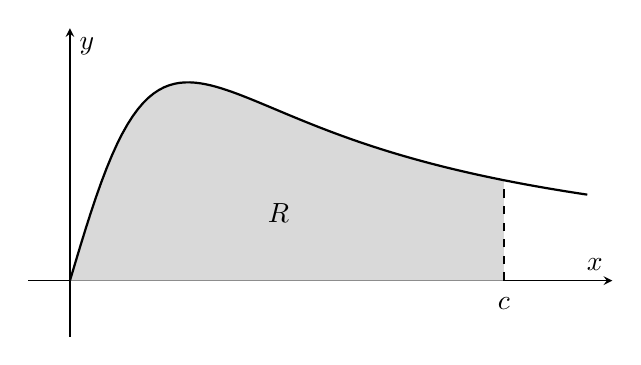
\begin{tikzpicture}
\begin{axis}[
  axis lines=middle,
  xlabel={$x$},
  ylabel={$y$},
  xmin=-0.5, xmax=6.5,
  ymin=-0.1, ymax=0.45,
  xtick=\empty,
  ytick=\empty,
  width=9cm, height=5.5cm,
  samples=100,
  domain=0:6.25,
  clip=false,
]
\addplot[name path=F, thick, domain=0:6.2] {x/(x^2+2)};
\addplot[name path=G, draw=none, domain=0:5.2] {0};
\addplot[thick, dashed] coordinates {(5.2, 0) (5.2, {5.2/(5.2^2+2)})};
\addplot[fill=black!15] fill between[of=F and G, soft clip={domain=0:5.2}];
\node at (axis cs:5.2, -0.04) {$c$};
\node at (axis cs:2.5, 0.12) {$R$};
\end{axis}
\end{tikzpicture}
\end{center}
\vspace{-0.3cm}

The shaded region $R$ is bounded by the curve, the $x$-axis and the line $x = c$.

The area of $R$ is $\ln 3$.

Find the value of $c$.

\begin{tikzpicture}
  \draw (-0.6,0) rectangle (11,7);
  \foreach \y in {1,2,...,6} \draw[dotted] (0,\y)--(10.5,\y);
\end{tikzpicture}

\end{enumerate}
\end{document}

Solutions
  Problem 1 — Arithmetic sequence:
  (a) u₁ + 3d = u₄ → 0.6 + 3d = 0.15 → d = -0.15
  (b) u₂ = 0.45, u₃ = 0.3, sum = (0.6 + 0.45 + 0.3 + 0.15)/k = 1 → k = 1.5

  Problem 2 — Pythagorean triple:
  (a) LHS = a² + (a⁴ - 2a² + 1)/4 = (4a² + a⁴ - 2a² + 1)/4 = (a⁴ + 2a² + 1)/4 = ((a²+1)/2)²
  (b) Area = ½ · a · (a²-1)/2 = a(a²-1)/4

  Problem 3 — Rational function:
  (a) 7x + 7 = 0 → x = -1
  (b)(i) x = 2  (ii) y = 7/2
  (c) x(2y-4) = 7y+7 → 2xy - 7y = 4x + 7 → f⁻¹(x) = (4x+7)/(2x-7)

  Problem 4 — Double angle:
  (a) cos2x = 1 - 2sin²x → 1 - 2sin²x = sinx → 2sin²x + sinx - 1 = 0
  (b) (2sinx - 1)(sinx + 1) = 0 → sinx = 1/2 or sinx = -1
      x = -π/2, π/6, 5π/6

  Problem 5 — Trig equation:
  θ = x/2 + π/3, cosθ = 1/√2, ref angle π/4
  θ = π/4 → x = -π/6 (rejected, negative)
  θ = 2π - π/4 = 7π/4 → x/2 = 7π/4 - π/3 = 17π/12 → x = 17π/6

  Problem 6 — Probability:
  (a) Independent: P(A∩B) = 0.3 × 0.8 = 0.24
  (b) P(A∪B) ≤ 1 → 1.1 - P(A∩B) ≤ 1 → min P(A∩B) = 0.1
  (c) A ⊆ B → max P(A∩B) = P(A) = 0.3

  Problem 7 — Antiderivative:
  y = sin(x - π/4) + c, sub x = 3π/4, y = 2:
  2 = sin(π/2) + c = 1 + c → c = 1
  y = sin(x - π/4) + 1

  Problem 8 — Common tangent:
  (a) f'(x) = -2(x - h)
  (b) g'(3) = e, f'(3) = -2(3-h) = e → h = (e+6)/2
  (c) f(3) = g(3): -(e/2)² + 2k = e + k → k = e + e²/4

  Problem 9 — Integration:
  ∫₀ᶜ x/(x²+2) dx, let u = x²+2:
  = ½ln(x²+2)|₀ᶜ = ½ln((c²+2)/2) = ln3
  ln((c²+2)/2) = ln9 → c²+2 = 18 → c = 4
